% Copyright 2004 by Till Tantau <tantau@users.sourceforge.net>.
%
% In principle, this file can be redistributed and/or modified under
% the terms of the GNU Public License, version 2.
%
% However, this file is supposed to be a template to be modified
% for your own needs. For this reason, if you use this file as a
% template and not specifically distribute it as part of a another
% package/program, I grant the extra permission to freely copy and
% modify this file as you see fit and even to delete this copyright
% notice. 

\documentclass{beamer}
%\usepackage[style=authoryear,backend=bibtex,useprefix=true]{biblatex}
\usepackage[style=authoryear,backend=biber,useprefix=true]{biblatex}
%\setbeamertemplate{navigation symbols}{}

\makeatletter
\let\@@magyar@captionfix\relax
\makeatother
\usepackage[utf8]{inputenc}


% only for this example, otherwise in .bib file
\usepackage{filecontents}

\bibliography{reference}
\usepackage{textcomp}
\usepackage{graphicx}
\usepackage[font=normalsize]{caption}
\usepackage{subcaption}
\graphicspath{ {./images/} }
\usepackage{color, colortbl}
\definecolor{Gray}{gray}{0.9}
\usepackage{biblatex}
\usepackage{float}
\usepackage{wrapfig}
\usepackage{amssymb}
\usepackage{amsmath}
\usepackage{amstext}
\usepackage{multirow}
\usepackage{url}
\usepackage{tabu}


\renewcommand{\footnotesize}{\tiny}
\newcommand{\notesize}{\fontsize{8}{10}\selectfont}
\usepackage[labelformat=empty]{caption}

\usepackage[linesnumbered,ruled]{algorithm2e}
\usepackage{multicol}
% There are many different themes available for Beamer. A comprehensive
% list with examples is given here:
% http://deic.uab.es/~iblanes/beamer_gallery/index_by_theme.html
% You can uncomment the themes below if you would like to use a different
% one:
%\usetheme{AnnArbor}
%\usetheme{Antibes}
%\usetheme{Bergen}
%\usetheme{Berkeley}
%\usetheme{Berlin}
%\usetheme{Boadilla}
%\usetheme{boxes}
%\usetheme{CambridgeUS}
%\usetheme{Copenhagen}
%\usetheme{Darmstadt}
%\usetheme{default}
%\usetheme{Frankfurt}
%\usetheme{Goettingen}
%\usetheme{Hannover}
%\usetheme{Ilmenau}
%\usetheme{JuanLesPins}
%\usetheme{Luebeck}
\usetheme{Madrid}
%\usetheme{Malmoe}
%\usetheme{Marburg}
%\usetheme{Montpellier}
%\usetheme{PaloAlto}
%\usetheme{Pittsburgh}
%\usetheme{Rochester}
%\usetheme{Singapore}
%\usetheme{Szeged}
%\usetheme{Warsaw}

\usepackage{filecontents}

\title{\large Building Resource Auto-Scaler with Functional-Link Neural Network and Adaptive Bacterial Foraging Optimization}

% A subtitle is optional and this may be deleted

%\author{\small Thieu Nguyen\inst{1} \and Binh Minh Nguyen\inst{1} \and \underline{Giang Nguyen}\inst{2}}
\author{\small Thieu Nguyen \and Minh Nguyen \and \underline{Giang Nguyen}}
% - Give the names in the same order as the appear in the paper.
% - Use the \inst{?} command only if the authors have different
%   affiliation.

%\institute[Universities of Somewhere and Elsewhere] % (optional, but mostly needed)
%{
%  \inst{1}%
%  School of Information and Communication Technology\\
%  Hanoi University of Science and Technology, Hanoi, Vietnam
%  \and
%  \inst{2}%
%  Institute of Informatics\\
%  Slovak Academy of Sciences, Bratislava, Slovakia}
% - Use the \inst command only if there are several affiliations.
% - Keep it simple, no one is interested in your street address.

\institute{ 
Hanoi University of Science and Technology, Hanoi, Vietnam\\
Institute of Informatics, Slovak Academy of Sciences, Bratislava, Slovakia}

\date{TAMC 2019\\
The 15th Annual Conference on \\Theory and Applications of Models of Computation }
% - Either use conference name or its abbreviation.
% - Not really informative to the audience, more for people (including
%   yourself) who are reading the slides online

\subject{Theoretical Computer Science}
% This is only inserted into the PDF information catalog. Can be left
% out. 

% If you have a file called "university-logo-filename.xxx", where xxx
% is a graphic format that can be processed by latex or pdflatex,
% resp., then you can add a logo as follows:

% \pgfdeclareimage[height=0.5cm]{university-logo}{university-logo-filename}
% \logo{\pgfuseimage{university-logo}}

% Delete this, if you do not want the table of contents to pop up at
% the beginning of each subsection:
\AtBeginSubsection[]
{
  \begin{frame}<beamer>{Outline}
    \tableofcontents[currentsection,currentsubsection]
  \end{frame}
}
\makeatletter
\setbeamertemplate{footline}{
	\leavevmode%
	\hbox{%
		\begin{beamercolorbox}[wd=.75\paperwidth,ht=2.2ex,dp=0.8ex,center]{author in head/foot}%
			\usebeamerfont{author in head/foot}\insertshortauthor
		\end{beamercolorbox}%
		\begin{beamercolorbox}[wd=.25\paperwidth,ht=2.2ex,dp=0.8ex,right]{date in head/foot}%
			\usebeamerfont{date in head/foot}\insertshortdate{}\hspace*{8em}*{2em}
			\insertframenumber{} / \inserttotalframenumber\hspace*{2.75ex} 
		\end{beamercolorbox}}%
		\vskip0pt%
	}
	\makeatother
\setbeamerfont{footline}{size=\fontsize{8}{10}\selectfont}

\begin{document}

\begin{frame}
  \titlepage
\end{frame}

\begin{frame}{Outline}
  \tableofcontents
  % You might wish to add the option [pausesections]
\end{frame}


\section{Motivation}
\begin{frame}{Motivation}
	\begin{itemize}
		\item {Cloud providers offer users a certain auto-scaling mechanism, which mainly operates based on predefined threshold resource usage\\ $\,\to\,$ Resource provision is often delayed and cant adapt the Quality of Service (QoS) for those applications. }
		\item {Applying predictive future usages to the clouds is still has barriers:} 
		\begin{itemize}
			\item Inaccuracy forecasting by only advanced in single metric over time
			\item The complexity of those model when deployed but keep the effectiveness in forecast 
			\item The prediction-based auto-scaling system also must have a scaling decision mechanism which ensures QoS defined in Service-Level Agreement (SLA) signed between cloud customers and vendors
		\end{itemize}
	\end{itemize}
\end{frame}

\section{Contributions}
\begin{frame}{Contributions}
	\begin{itemize}
		\item {Applying a novel variant of FLNN which is trained by adaptive bacterial foraging optimization with life-cycle and social learning  to build a new approach for proactive auto-scaling problem in clouds (called FLAB)}
		\item {Using SLA-awareness to make decision as well as evaluate scaling decision in our auto-scaler }
		\item {Testing the proposed system performance with real dataset produced by Google cluster}
	\end{itemize}
\end{frame}


\section{Related works}
\begin{frame}{ Forecast models for cloud computing}
	\begin{itemize}
			\item{
				Time series forecasting ~\footcite{Hipel et al. 1994}
				}
				\begin{itemize}
					\item {
						Autoregressive (AR), moving average (MA), exponential smoothing, error-trend-seasonal (ETS), automated autoregressive integrated moving average (ARIMA) and back-propagation NN  
					}
				\end{itemize}	

			\item {
	 			Multi-layer neural network (MLNN) model for prediction URL resource requests of a WWW server at NASA and at EPA~\footcite{Prevost et al. 2011}  
			}
	\end{itemize}
	\vspace{0.3cm}
		$\,\to\,$ Experimental solution with simpler structure\\
		$\,\to\,$ Multivariate model: system overview, hidden relationships
%		$\,\to\,$ Still considered the problem with univariate time series.
\end{frame}


%\begin{frame}{Functional-link neural network}
%	\begin{itemize}
%		\item{
%			 \small FLNN has a flat architecture with a single neuron and predefined basis functions (Pao et al.\footcite{Yoh-Han Pao 1989}). By removing the hidden layers without giving up non-linerity by providing the input layer with expanded inputs. The authors reported their advantages: 
%			\begin{itemize}
%				\item {
%					\small Less computational cost in comparison with MLP in pattern-recognition task.
%				}
%				\item {
%					\small Easily implemented in hardware applications
%				}
%			\end{itemize}
%		}
%		\item{
%			\small  Successful in e.g., stock market \footcite{Majhi et al. 2009} and exchange rate prediction \footcite{Majhi et al. 2012}
%		}
%		\item{
%			\small  Comparable accuracy with MLNN (DL) and computation time aspects \footcite{Khandelwal et al. 2015, Sahoo et al. 2018}
%		}		
%	\end{itemize}
%	
%	$\,\to\,$ FLNN approach: still using back-propagation (BP) with gradients descent \footcite{Dehuri, Satchidananda, and Sung-Bae Cho 2010}
%\end{frame}

\begin{frame}{Functional-link neural network (Expansion functions)}

\begin{table}[h]
	\begin{center}
		\begin{tabu}{| c | c| c | c | c | c | c | c |}
			\hline
Name & Polynomial functions \\
\hline
\multirow{2}*{}{Chebyshev$^1$} & $T_0(x) = 1$, $T_1(x) = x$ \\ 
& $T_{n+1} = 2xT_n(x) - T_{n-1}(x) $\\ \hline

\multirow{2}{*}{Legendre$^1$} & $ P_0(x) = 1, P_1(x) = x $ \\
& $ (n+1)P_{n+1}(x) = (2n+1)x P_n(x) - nP_{n-1}(x) $ \\ \hline

\multirow{3}{*}{Laguerre$^1$} & $L_0(x) = 1$, $L_1(x) = 1 - x$ \\
& $L_{k+1}(x) = \displaystyle \frac{(2k+1-x)L_k(x) - kL_{k-1}(x)}{k+1}$ \\ \hline

\multirow{1}{*}{Power Series$^1$} & $\displaystyle \sum_{n=0}^{\infty} a_n(x-c)^n = a_0 + a_1(x-c)^1 + a_2(x-c)^2 + ... $ \\  \hline

\multirow{1}{*}{Trigonometric$^1$} & $\displaystyle T(x) = a_0 + \sum_{n=1}^{N}a_ncos(nx) + i \sum_{n=1}^{N} b_nsin(nx) $ \\ \hline
		\end{tabu}
		\label{table:forecasting_results_MLNN_FLNN_FLGANN}
	\end{center}
\end{table}

[1]: Wikipedia

\end{frame}



\begin{frame}{Adaptive Bacterial Foraging Optimization (ABFOLS)}
	\begin{itemize}
		\item{
			\small BFO is an evolutionary computing technique based on principle of bacterial movement (i.e. tumbling, swimming or repositioning) to food-seeking \footcite{Passino et al. 2002}
		}
		\item {
			\small Unfortunately, BFO has certain shortages e.g., the appropriate time and method for dispersal and reproduction must be carefully selected, otherwise the stability of population may be destroyed \footcite{Yan et al. 2012}.		
		}		
		\item{
			\small 
			 The authors of \footcite{Yan et al. 2012} proposed an improvement for BFO including life-cycle of bacteria, social learning and adaptive search step length (ABFOLS) offer significant improvements over BFO in complexity and competitive performances as compared with other algorithms (e.g. GA) on higher-dimensional problems. 
		}
	\end{itemize}
	$\,\to\,$ Experiment: use ABFOLS to train FLNN instead of BP
\end{frame}


\begin{frame}{Cloud resources provision under SLA conditions}
	\begin{itemize}
		\item{
			\small The authors \footcite{Reig et al. 2010} presented a job scheduling system using machine learning to predict workloads and allocate resources complying with SLA 
		}
		\item {
			\small The authors of \footcite{Souza et al. 2015} used SLA to estimate the amount of resources required for making scaling actions.
		}		
		\item{
			\small Both papers above still operate based on single workload metric such as CPU usage, response time,...
		}
		\item{
			\small The work \footcite{Tran et al. 2017} allows processing multiple metrics, SLA violation still is evaluated based on resource usages (e.g. CPU, and memory usage)
		}
	\end{itemize}
	$\,\to\,$ Our study: Assess SLA to ensure QoS using the number of provided virtual machines (VMs)
\end{frame}



%\begin{frame}{Multivariate time-series problem}
%	\begin{itemize}
%		\item{
%			\small The authors proposed MF-GABPNN model to mine the relationship among different metric types in forecast process. \footcite{Tran et al. 2017}
%		}
%		\item{
%			\small The analytics of relation among different metric types has been exposed and implemented in their prediction models.\footcite{Tran et al. 2018}
%		}
%	\end{itemize}
%	$\,\to\,$ There are no works, which use FLNN for multivariate time-series data prediction problem.
%\end{frame}


%\section{Designing system architecture}
%\begin{frame}{System architecture}
%	\begin{figure}
%		\centering
%		\includegraphics[scale=0.42]{FLGANN_system.pdf}
%		\caption*{Proposed architecture of resources forecasting system}
%		\label{fig:overall}
%	\end{figure}
%\end{frame}

\subsection{Extraction phase}
\begin{frame}{Extraction phase}
	\begin{figure}
		\centering
		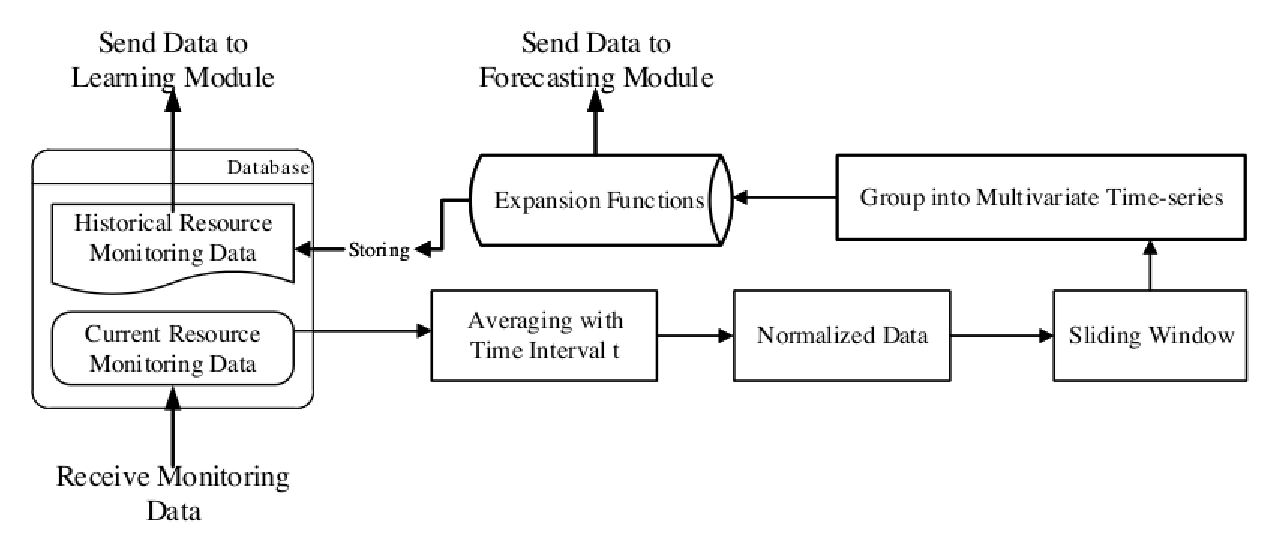
\includegraphics[width=0.75 \textwidth]{true/Extraction_Module.eps} %[width=9cm,height=5cm]
		\label{fig:preprocessing}			
	\end{figure}
	\begin{itemize}
		\item{Construct suitable dataset for the learning part in our system }
		\begin{itemize}
			\item {\notesize Using collected raw monitoring data from the underlying Cloud System.}
			\item{\notesize Values of each cloud monitoring metric are transformed into the corresponding time series $r_i(t)$ ($i = 1, 2, \ldots, M$) with time interval $\tau$}
			\item{\notesize Averaging values of given metrics in the given interval of $\rho$ for each point in time series $r_i(t)$}
			\vspace{0.2cm}
			\item{\notesize Normalization, which scales a time series in the range of [0, 1]}
			\vspace{0.2cm}
			\item{\notesize Time-series data is transformed to supervised data by using sliding method.}
			\vspace{0.2cm}
			\item{\notesize Single multivariate data which is created by group all resource metric types.}
			\vspace{0.2cm}
			\item{\notesize Function Expansions such as Chebyshev, Legendre or Power help network has ability of catching the nonlinear relationship between the inputs and outputs.}
		\end{itemize}
	\end{itemize}
\end{frame}

\subsection{Learning phase}
\begin{frame}{Learning phase}

\begin{figure}
		\centering
		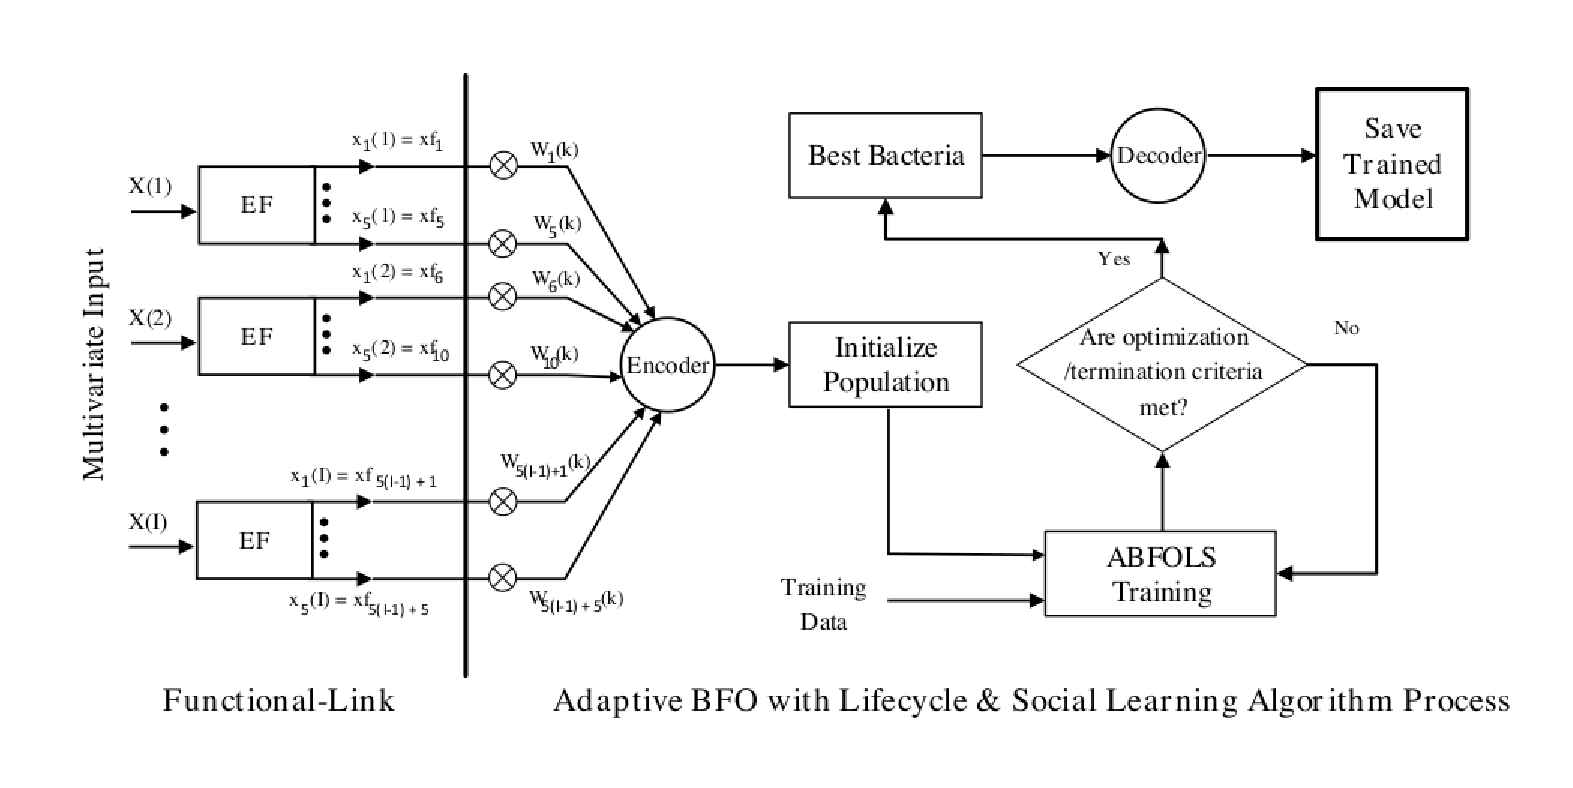
\includegraphics[width=0.8 \textwidth]{true/FLBFONN_training.eps} %[width=9cm,height=5cm]
		\caption*{\notesize Figure 1: FLABL training process}
		\label{fig:preprocessing}			
\end{figure}
	\begin{itemize}
		\item{\notesize Encoder component is used to encode the weights and bias of network into a chromosome (real-value vector). }
		\item{ \notesize Decoder component decodes the chromosome into the weights and bias of network. }
	\end{itemize}
	
\end{frame}


\subsection{Scaling phase}
\begin{frame}{Scaling phase}
\begin{figure}
		\centering
		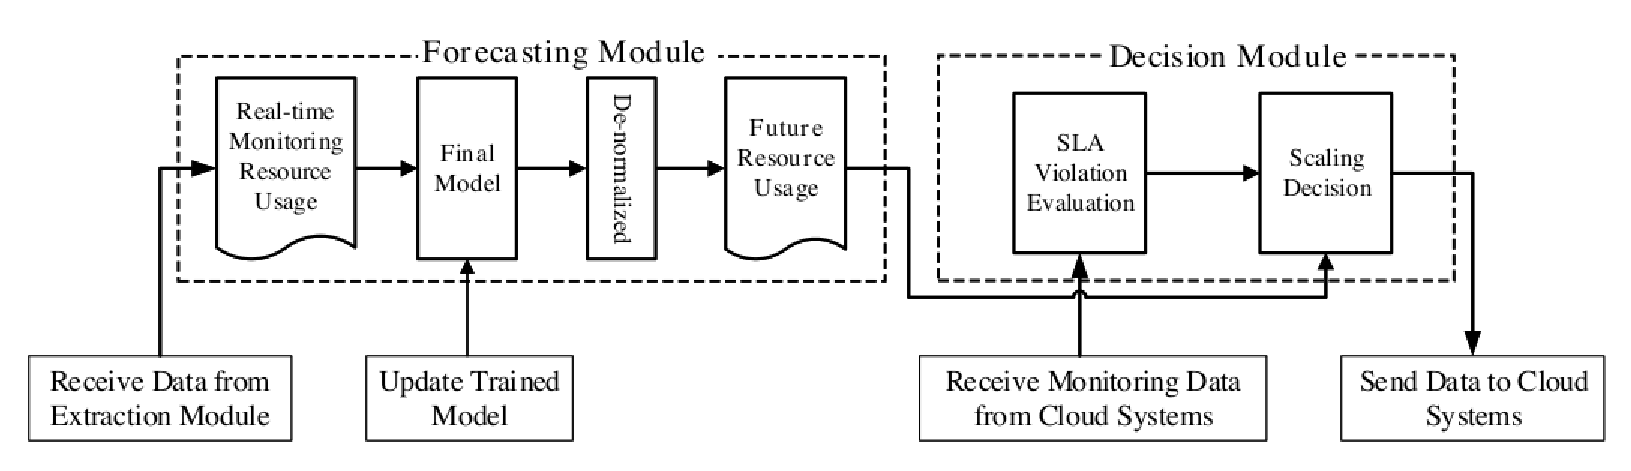
\includegraphics[width=0.8 \textwidth]{true/Forecasting_Module.eps} %[width=9cm,height=5cm]
		\caption*{\notesize Figure 1: Scaling phase}
		\label{fig:scaling_phase}			
\end{figure}

	\begin{itemize}
		\item{\notesize Forecasting module: using trained model to predicte new values. }
		\item{ \notesize Decision module: calculating the number of provided VMs based on the predictive resource comsumption. Our develop formula operates on the number of Vms allocated at previous time and with the VM numbers predicted in the future to decide the how many Vms will be provisioned as in equations 10, 11, 12.}
	\end{itemize}
\end{frame}


\subsection*{Scaling phase}
\begin{frame}{FLABL-based forecasting algorithm}
	\begin{figure}
		\includegraphics[width=0.45 \textwidth]{/true/forecasting_algorithm.png} %[width=9cm,height=5cm]
		\label{fig:ga}			
	\end{figure}
\end{frame}

	
\subsection*{Scaling phase}
\begin{frame}{SLA-based scaling algorithm}
	\begin{figure}
		\includegraphics[width=0.85 \textwidth]{true/scaling_algorithm.png} %[width=9cm,height=5cm]
		\label{fig:scaling_algorithm}			
	\end{figure}
\end{frame}





\section{Experiments}
\subsection{Experimental setup}
\begin{frame}{Dataset}
	\frametitle{Data set}
	\begin{itemize}
		\item {
			Data set: Google cluster trace dataset
			\begin{itemize}
			\item 20 metrics which are measured by several metrics such as CPU, memory usage, disk I/O mean time, and so forth
			\item 12O32799308 data items in data set
			\item  Less than 2\% of jobs that run longer than one day, even though such jobs contribute to over 80\% of the dataset records
			\item A long-running job with ID 6176858948 that consists of 25954362 monitoring data items during the 29-day period
			\item Used dataset from 1st to 20th day to train model and from 21st to 29th to evaluate the model performance.
			\end{itemize}
		}
		\item{
			The health function in ABFO: \newline
			$Health = RMSE = \sqrt{  \frac{\sum_{i=1}^N( forecast(i) - actual(i) )^2}{N} }	\label{eq_fitness} $. 
			}
	\end{itemize}
\end{frame}

\subsection*{Experimental setup}
\begin{frame}{SLA evaluation mechanisms}
	\frametitle{SLA evaluation mechanisms}
	\begin{itemize}
		\item {
			SLAVTP (SLA Violation Time Percentage) \footcite{Tran et al. 2017}: to evaluate our proposed VM calculation mechanism
			\begin{itemize}
			\item $ SLAVTP = \frac{T_{under-provisioning}}{T_{execution}}$, where 
			\item $T_{under-provisioning}$ is the time when at least one allocation resource causes "under-provisioning" (i.e. lack of RAM or CPU core), and 
			\item $T_{execution}$ is total time of the application running in cloud system. 
			\end{itemize}
		}
		\item{
			ADI(Auto-scaling Demand Index) \footcite{Netto et al. 2014} the difference between actual and desired resource utilization. \newline
			Or, the total distance between $u_t$ and $[L, U]$. ($u_t$ is the utilization level of the system, $L$ and $U$ correspond to the lower and upper limits of reasonable resource use, with $0 \le L \le U \le 1.0$)
			\begin{itemize}
			\item The optimization strategy will gield a minimum of $\sigma = \sum_{t \in T}{\sigma_t}$ where, $\sigma_t = L - u_t$ if $u_t \le L$; $\sigma_t = 0$ if $L < u_t <U$; $\sigma_t = u_t -U$ if otherwise. 
			\end{itemize}
		}
	\end{itemize}
\end{frame}



\subsection{Forecasting Resource Consumption}
\begin{frame}{FLABL forecast accuracy}
	\begin{figure}
		\includegraphics[width=0.9 \textwidth]{true/forecasting_results.png} %[width=9cm,height=5cm]
		\label{fig:forecasting_results}			
	\end{figure}
\end{frame}


\begin{frame}{FLABL forecast accuracy}
	\begin{figure}
		\centering
		\begin{subfigure}{0.5\textwidth}
			\centering
			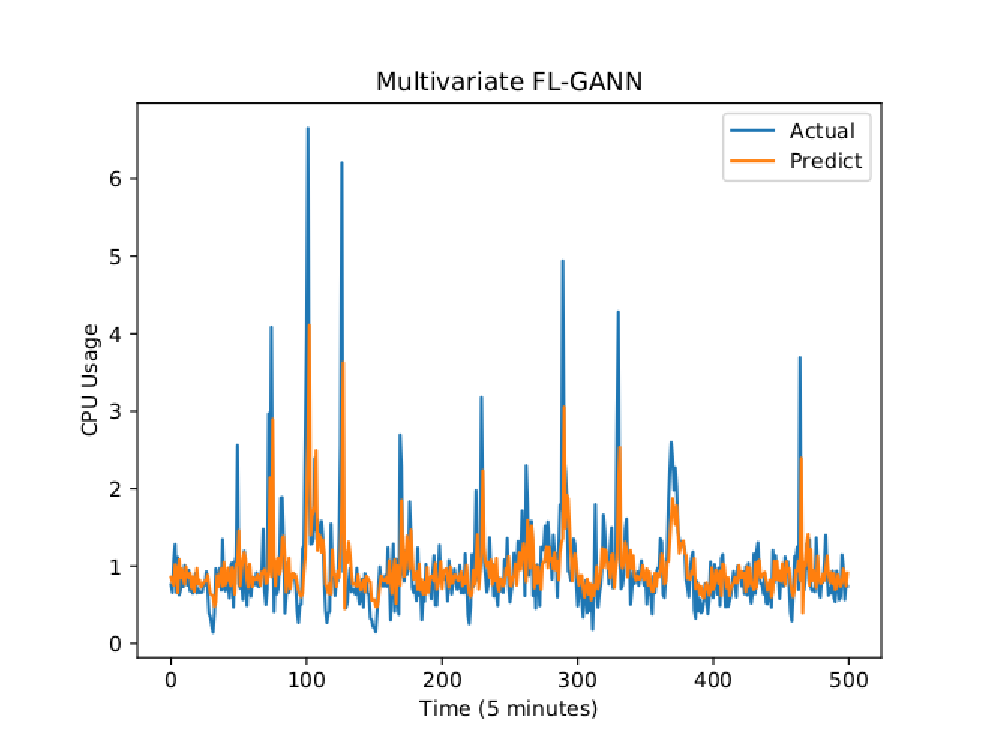
\includegraphics[width=1.0\linewidth]{true/multi_cpu_flgann.eps}
			\label{fig:sub11}
		\end{subfigure}%
		\begin{subfigure}{.5\textwidth}
			\centering
			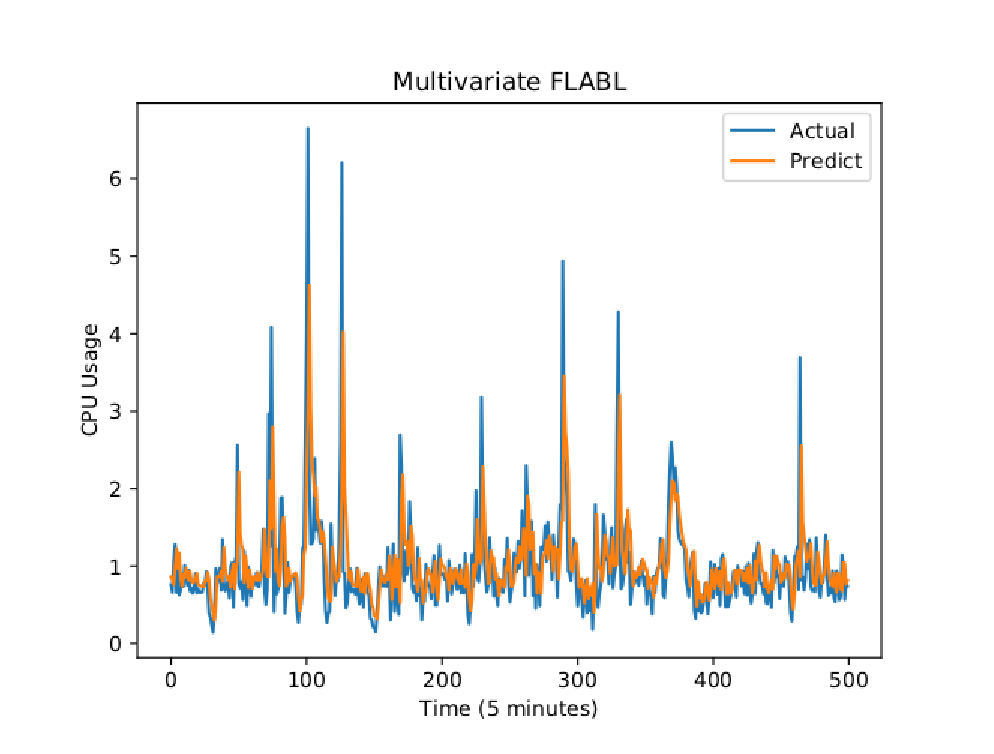
\includegraphics[width=1.0\linewidth]{true/multi_cpu_flabl.eps}
			\label{fig:sub21}
		\end{subfigure}%
		\caption{CPU usage of FL-GANN model(left) and FLABL(right) with multivariate data}
		\label{fig:cpu_predict}
	\end{figure}
\end{frame}


\begin{frame}{FLABL forecast accuracy}
	\begin{figure}
		\centering
		\begin{subfigure}{0.5\textwidth}
			\centering
			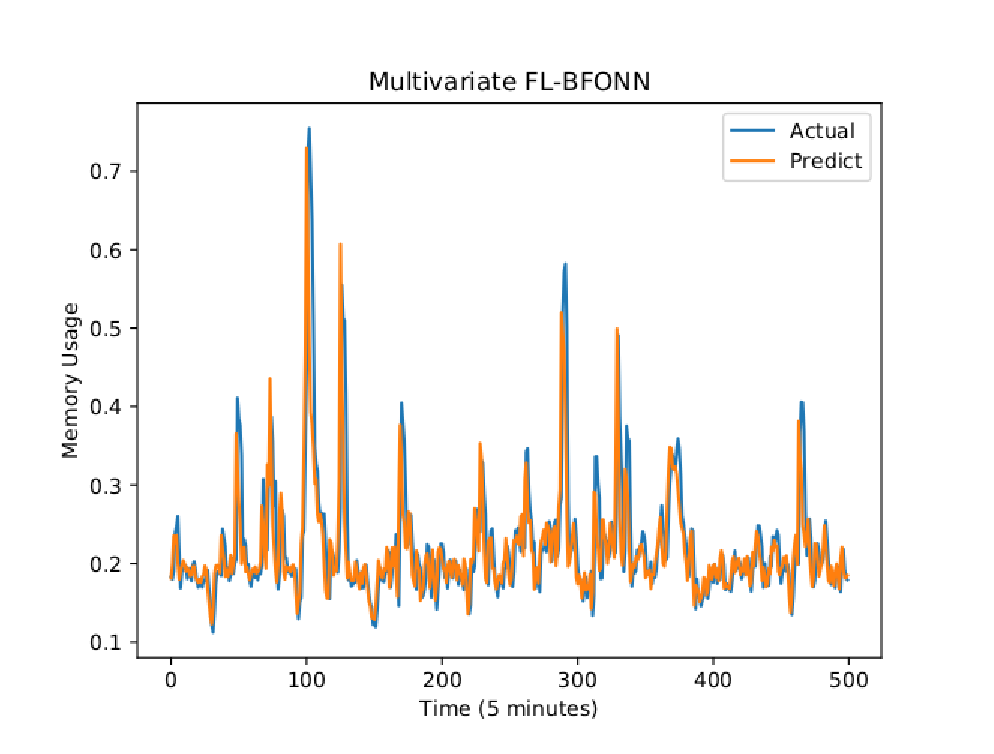
\includegraphics[width=1.0\linewidth]{true/multi_ram_flbfonn.eps}
			\label{fig:sub11}
		\end{subfigure}%
		\begin{subfigure}{.5\textwidth}
			\centering
			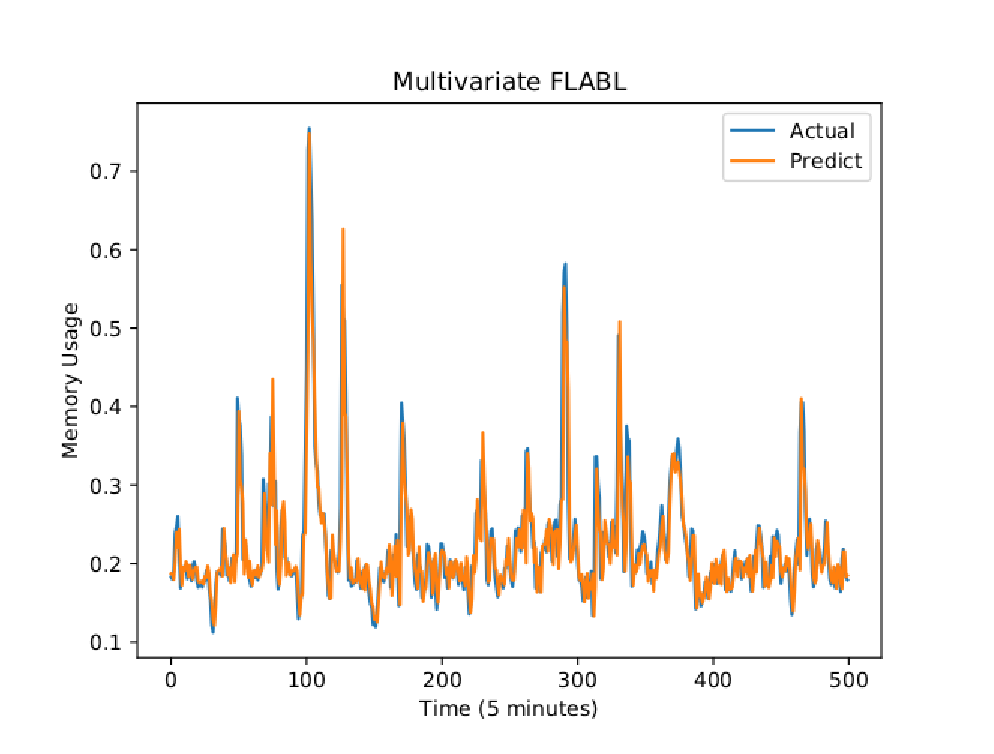
\includegraphics[width=1.0\linewidth]{true/multi_ram_flabl.eps}
			\label{fig:sub21}
		\end{subfigure}%
		\caption{Memory usage of FL-BFONN model(left) and FLABL(right) with multivariate data}
		\label{fig:cpu_predict}
	\end{figure}
\end{frame}


\begin{frame}{FLABL runtime}
	\begin{figure}
		\includegraphics[width=1.0 \textwidth]{true/system_runtime.png} %[width=9cm,height=5cm]
		\label{fig:forecasting_results}			
	\end{figure}
\end{frame}









\subsection{Auto-scaling strategy}
\begin{frame}{The lack of resources provision - SLAVTP}
	\begin{figure}
		\includegraphics[width=1.0 \textwidth]{true/auto_scaler1.png} %[width=9cm,height=5cm]
		\label{fig:forecasting_results}			
	\end{figure}
\end{frame}


\begin{frame}{The over-provision of resources provision - ADI}
	\begin{figure}
		\includegraphics[width=1.0 \textwidth]{true/auto_scaler2.png} %[width=9cm,height=5cm]
		\label{fig:forecasting_results}			
	\end{figure}
\end{frame}


\begin{frame}{The number of predicted, allocated, used VMs }
	\begin{figure}
		\includegraphics[width=1.0 \textwidth]{true/vms.png} %[width=9cm,height=5cm]
		\label{fig:forecasting_results}		
		\caption{The number of predicted, allocated, used VMs with sliding window = 3, adaptation length L = 5, and scaling coefficient s = 1 (left), s = 1.3(right)}	
	\end{figure}
\end{frame}


\section{Conclusion and future work}
\begin{frame}{Conclusion and future work}
	\begin{itemize}
		\item {
		Proposed a complete cloud proactive auto-scaler with complete modules from prediction to decision making.
		}
		\item{
			Several mechanisms to improve accuracy as well as effectiveness of the resource usage prediction model using
			\begin{itemize}
			\item {
				Applying adaptive bacterial foraging life-cycle and social learning optimization with the simple functional-link neural network (called FLABL)
			}
			\item {
				Proposing an auto-scaler which be able to analyzing multiple monitoring metrics at the same time.
			}
			\end{itemize}
		}
		\item {
			Proposing an efficient way to calculate the number of Vms provided for cloud-based applications using SLA violation measurement in decision module.
		}
	\end{itemize}
\end{frame}

\begin{frame}{}
	
		\centering \Huge
		\emph{Thank you for your attention!!!}
			
		
\end{frame}
%\label{sect:bib}
%\bibliographystyle{plain}
%\bibliography{reference}
\end{document}


